% GNUPLOT: LaTeX picture with Postscript
\begingroup
  \fontfamily{cmss}%
  \selectfont
  \makeatletter
  \providecommand\color[2][]{%
    \GenericError{(gnuplot) \space\space\space\@spaces}{%
      Package color not loaded in conjunction with
      terminal option `colourtext'%
    }{See the gnuplot documentation for explanation.%
    }{Either use 'blacktext' in gnuplot or load the package
      color.sty in LaTeX.}%
    \renewcommand\color[2][]{}%
  }%
  \providecommand\includegraphics[2][]{%
    \GenericError{(gnuplot) \space\space\space\@spaces}{%
      Package graphicx or graphics not loaded%
    }{See the gnuplot documentation for explanation.%
    }{The gnuplot epslatex terminal needs graphicx.sty or graphics.sty.}%
    \renewcommand\includegraphics[2][]{}%
  }%
  \providecommand\rotatebox[2]{#2}%
  \@ifundefined{ifGPcolor}{%
    \newif\ifGPcolor
    \GPcolortrue
  }{}%
  \@ifundefined{ifGPblacktext}{%
    \newif\ifGPblacktext
    \GPblacktextfalse
  }{}%
  % define a \g@addto@macro without @ in the name:
  \let\gplgaddtomacro\g@addto@macro
  % define empty templates for all commands taking text:
  \gdef\gplbacktext{}%
  \gdef\gplfronttext{}%
  \makeatother
  \ifGPblacktext
    % no textcolor at all
    \def\colorrgb#1{}%
    \def\colorgray#1{}%
  \else
    % gray or color?
    \ifGPcolor
      \def\colorrgb#1{\color[rgb]{#1}}%
      \def\colorgray#1{\color[gray]{#1}}%
      \expandafter\def\csname LTw\endcsname{\color{white}}%
      \expandafter\def\csname LTb\endcsname{\color{black}}%
      \expandafter\def\csname LTa\endcsname{\color{black}}%
      \expandafter\def\csname LT0\endcsname{\color[rgb]{1,0,0}}%
      \expandafter\def\csname LT1\endcsname{\color[rgb]{0,1,0}}%
      \expandafter\def\csname LT2\endcsname{\color[rgb]{0,0,1}}%
      \expandafter\def\csname LT3\endcsname{\color[rgb]{1,0,1}}%
      \expandafter\def\csname LT4\endcsname{\color[rgb]{0,1,1}}%
      \expandafter\def\csname LT5\endcsname{\color[rgb]{1,1,0}}%
      \expandafter\def\csname LT6\endcsname{\color[rgb]{0,0,0}}%
      \expandafter\def\csname LT7\endcsname{\color[rgb]{1,0.3,0}}%
      \expandafter\def\csname LT8\endcsname{\color[rgb]{0.5,0.5,0.5}}%
    \else
      % gray
      \def\colorrgb#1{\color{black}}%
      \def\colorgray#1{\color[gray]{#1}}%
      \expandafter\def\csname LTw\endcsname{\color{white}}%
      \expandafter\def\csname LTb\endcsname{\color{black}}%
      \expandafter\def\csname LTa\endcsname{\color{black}}%
      \expandafter\def\csname LT0\endcsname{\color{black}}%
      \expandafter\def\csname LT1\endcsname{\color{black}}%
      \expandafter\def\csname LT2\endcsname{\color{black}}%
      \expandafter\def\csname LT3\endcsname{\color{black}}%
      \expandafter\def\csname LT4\endcsname{\color{black}}%
      \expandafter\def\csname LT5\endcsname{\color{black}}%
      \expandafter\def\csname LT6\endcsname{\color{black}}%
      \expandafter\def\csname LT7\endcsname{\color{black}}%
      \expandafter\def\csname LT8\endcsname{\color{black}}%
    \fi
  \fi
    \setlength{\unitlength}{0.0500bp}%
    \ifx\gptboxheight\undefined%
      \newlength{\gptboxheight}%
      \newlength{\gptboxwidth}%
      \newsavebox{\gptboxtext}%
    \fi%
    \setlength{\fboxrule}{0.5pt}%
    \setlength{\fboxsep}{1pt}%
    \definecolor{tbcol}{rgb}{1,1,1}%
\begin{picture}(8640.00,5760.00)%
    \gplgaddtomacro\gplbacktext{%
      \csname LTb\endcsname%%
      \put(300,1440){\makebox(0,0)[r]{\strut{}$0.2$}}%
      \put(300,1972){\makebox(0,0)[r]{\strut{}$0.4$}}%
      \put(300,2503){\makebox(0,0)[r]{\strut{}$0.6$}}%
      \put(300,3035){\makebox(0,0)[r]{\strut{}$0.8$}}%
      \put(300,3566){\makebox(0,0)[r]{\strut{}$1$}}%
      \put(300,4098){\makebox(0,0)[r]{\strut{}$1.2$}}%
      \put(300,4629){\makebox(0,0)[r]{\strut{}$1.4$}}%
      \put(662,1220){\makebox(0,0){\strut{}$-0.25$}}%
      \put(1238,1220){\makebox(0,0){\strut{}$0$}}%
      \put(1814,1220){\makebox(0,0){\strut{}$0.25$}}%
      \put(2390,1220){\makebox(0,0){\strut{}$0.5$}}%
    }%
    \gplgaddtomacro\gplfronttext{%
      \csname LTb\endcsname%%
      \put(2699,610){\makebox(0,0)[r]{\strut{}Ag}}%
      \csname LTb\endcsname%%
      \put(2699,390){\makebox(0,0)[r]{\strut{}Au}}%
      \csname LTb\endcsname%%
      \put(3818,610){\makebox(0,0)[r]{\strut{}Cu}}%
      \csname LTb\endcsname%%
      \put(3818,390){\makebox(0,0)[r]{\strut{}Ir}}%
      \csname LTb\endcsname%%
      \put(4937,610){\makebox(0,0)[r]{\strut{}Ni}}%
      \csname LTb\endcsname%%
      \put(4937,390){\makebox(0,0)[r]{\strut{}Pd}}%
      \csname LTb\endcsname%%
      \put(6056,610){\makebox(0,0)[r]{\strut{}Pt}}%
      \csname LTb\endcsname%%
      \put(6056,390){\makebox(0,0)[r]{\strut{}Rh}}%
      \csname LTb\endcsname%%
      \put(-305,3167){\rotatebox{-270.00}{\makebox(0,0){\strut{}Activation Free Energy $\Delta G^\ddag$ (eV)}}}%
      \put(1583,890){\makebox(0,0){\strut{}$\Delta G_H$ (eV)}}%
      \colorrgb{0.00,0.00,0.00}%%
      \put(1653,3513){\rotatebox{28.90}{\makebox(0,0)[l]{\strut{}\tiny{Volmer, $R^2 = 0.68$}}}}%
      \colorrgb{0.90,0.12,0.06}%%
      \put(1814,2902){\rotatebox{-46.50}{\makebox(0,0)[l]{\strut{}\tiny{Heyrovsky, $R^2 = 0.79$}}}}%
      \colorrgb{0.00,0.45,0.70}%%
      \put(1814,3354){\rotatebox{5.30}{\makebox(0,0)[l]{\strut{}\tiny{Tafel, $R^2 = 0.03$}}}}%
    }%
    \gplgaddtomacro\gplbacktext{%
      \csname LTb\endcsname%%
      \put(3036,1440){\makebox(0,0)[r]{\strut{}}}%
      \put(3036,1972){\makebox(0,0)[r]{\strut{}}}%
      \put(3036,2503){\makebox(0,0)[r]{\strut{}}}%
      \put(3036,3035){\makebox(0,0)[r]{\strut{}}}%
      \put(3036,3566){\makebox(0,0)[r]{\strut{}}}%
      \put(3036,4098){\makebox(0,0)[r]{\strut{}}}%
      \put(3036,4629){\makebox(0,0)[r]{\strut{}}}%
      \put(3168,1220){\makebox(0,0){\strut{}$-1$}}%
      \put(3744,1220){\makebox(0,0){\strut{}$-0.5$}}%
      \put(4320,1220){\makebox(0,0){\strut{}$0$}}%
      \put(4895,1220){\makebox(0,0){\strut{}$0.5$}}%
      \put(5471,1220){\makebox(0,0){\strut{}$1$}}%
    }%
    \gplgaddtomacro\gplfronttext{%
      \csname LTb\endcsname%%
      \put(2937,3167){\rotatebox{-270.00}{\makebox(0,0){\strut{}}}}%
      \put(4319,890){\makebox(0,0){\strut{}$U_{PZC}$ vs SHE (V)}}%
      \colorrgb{0.00,0.00,0.00}%%
      \put(4527,2716){\rotatebox{-38.00}{\makebox(0,0)[l]{\strut{}\tiny{Volmer, $R^2 = 0.80$}}}}%
      \colorrgb{0.90,0.12,0.06}%%
      \put(4435,3779){\rotatebox{49.09}{\makebox(0,0)[l]{\strut{}\tiny{Heyrovsky, $R^2 = 0.66$}}}}%
      \colorrgb{0.00,0.45,0.70}%%
      \put(4607,3194){\rotatebox{-20.79}{\makebox(0,0)[l]{\strut{}\tiny{Tafel, $R^2 = 0.33$}}}}%
    }%
    \gplgaddtomacro\gplbacktext{%
      \csname LTb\endcsname%%
      \put(5772,1440){\makebox(0,0)[r]{\strut{}}}%
      \put(5772,1972){\makebox(0,0)[r]{\strut{}}}%
      \put(5772,2503){\makebox(0,0)[r]{\strut{}}}%
      \put(5772,3035){\makebox(0,0)[r]{\strut{}}}%
      \put(5772,3566){\makebox(0,0)[r]{\strut{}}}%
      \put(5772,4098){\makebox(0,0)[r]{\strut{}}}%
      \put(5772,4629){\makebox(0,0)[r]{\strut{}}}%
      \put(6233,1220){\makebox(0,0){\strut{}$-0.5$}}%
      \put(6781,1220){\makebox(0,0){\strut{}$0$}}%
      \put(7330,1220){\makebox(0,0){\strut{}$0.5$}}%
      \put(7878,1220){\makebox(0,0){\strut{}$1$}}%
    }%
    \gplgaddtomacro\gplfronttext{%
      \csname LTb\endcsname%%
      \put(5673,3167){\rotatebox{-270.00}{\makebox(0,0){\strut{}}}}%
      \put(7055,890){\makebox(0,0){\strut{}$\Delta G_H -\frac{b}{a}(U_{PZC})$}}%
      \colorrgb{0.00,0.00,0.00}%%
      \put(6233,1599){\rotatebox{56.78}{\makebox(0,0)[l]{\strut{}\tiny{Volmer, $R^2 = 0.96$}}}}%
      \colorrgb{0.90,0.12,0.06}%%
      \put(6123,4842){\rotatebox{-70.91}{\makebox(0,0)[l]{\strut{}\tiny{Heyrovsky, $R^2 = 0.96$}}}}%
      \colorrgb{0.00,0.45,0.70}%%
      \put(7220,3380){\rotatebox{21.04}{\makebox(0,0)[l]{\strut{}\tiny{Tafel, $R^2 = 0.16$}}}}%
    }%
    \gplbacktext
    \put(0,0){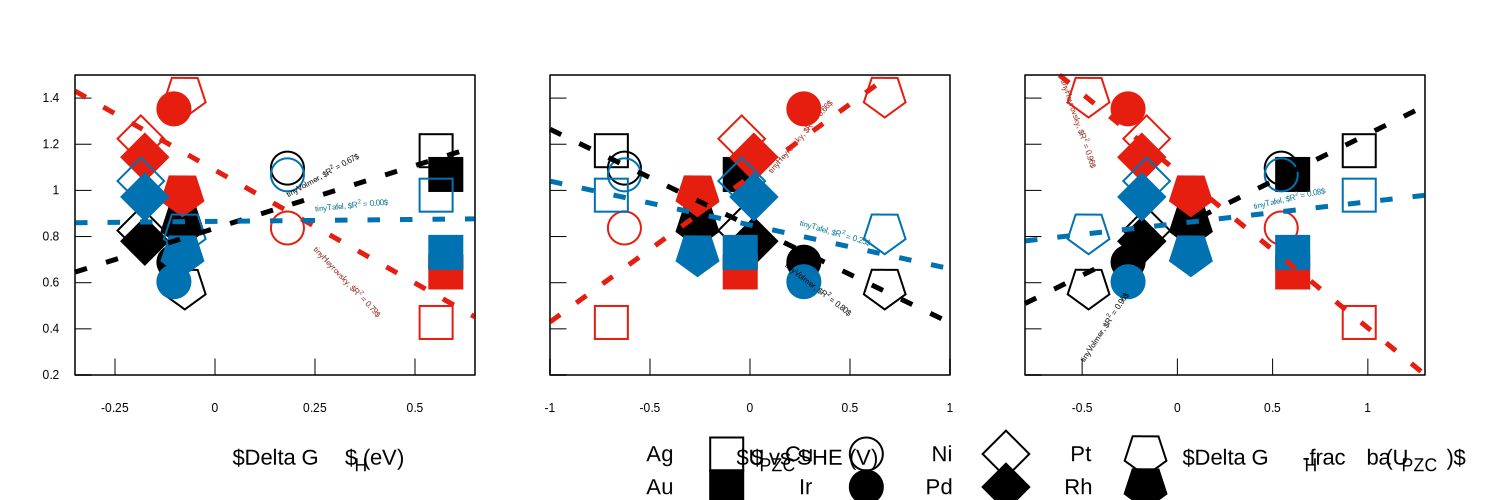
\includegraphics[width={432.00bp},height={288.00bp}]{NewVolcano}}%
    \gplfronttext
  \end{picture}%
\endgroup
